\section{\sout{Gradient descent}}
Uno de los puntos clave del aprendizaje de máquina supervisado es
definir una función objetivo que deberá ser optimizada durante el
proceso de aprendizaje. Esta función objetivo usualmente es una
\textit{función de costo} que se quiere minimizar. En el caso de
Adaline, se define la función de costos $J$ como la \textbf{Suma de
  los errores cuadrados (SSE)} entre la salida calculada y el valor
real.
\begin{equation}
  J(w)=1/2 \sum_i (y^{(i)} - \phi (z^{(i)}))^2
\end{equation}

La principal ventaja de esta función lineal de activación es que,
en contraste con la función escañón, la función de costos se vuelve
diferenciable. Otra propiedad de esta función de costos es que es
convexa. Así, es posible usar un algoritmo llamado \textit{gradient descent}
para encontrar los pesos que minimizan la función de costos, maximizando así
la \sout{accuracy} de las predicciones.

La idea detrás del gradient descent es disminuir el gradiente hasta encontrar
un mínimo (local o global) de la función de costo. En cada iteración, se reduce
un \textit{paso} del gradiente, donde cada \textit{paso} está determinado por
el valor del índice de aprendizaje, así como por la pendiente del gradiente.

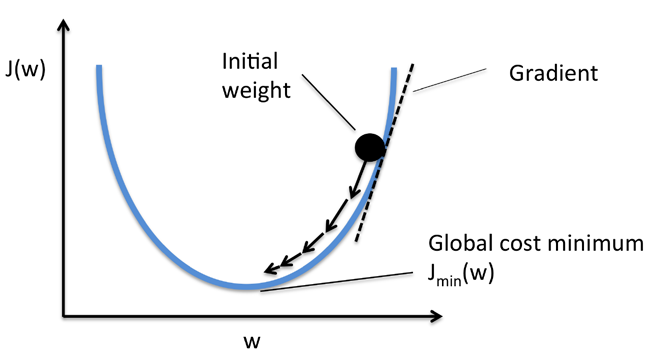
\includegraphics[scale=0.5]{gradient-descent}

Usando el \sout{gradient descent}, se pueden actualizar los pesos quitandole un \textit{paso}
al gradiente $\nabla J(w)$ de la función de costos $J(w)$:
\begin{equation}
  w := w + \Delta w
\end{equation}

En donde el cambio de peso $\Delta w$ se define como el gradiente negativo multiplicado
por el índice de aprendizaje $\eta$:
\begin{equation}
  \Delta w := -\eta \Delta J(w)
\end{equation}

Calculamos la derivada parcial de la función de costos SSE con respecto al
j-ésimo peso de la siguiente manera:
\begin{equation*}
\begin{split}
  \frac{\partial J}{\partial w_j} &= \frac{\partial}{\partial w_j}\frac{1}{2}\sum_i (y^{(i)} - \phi(z^{(i)}))^2 \\
  &= \frac{1}{2}\sum_i 2(y^{(i)} - \phi(z^{(i)}))\frac{\partial}{\partial w_j}(y^{(i)} - \phi(z^{(i)}))\\
  &= \sum_i (y^{(i)} - \phi(z^{(i)}))\frac{\partial}{\partial w_j}(y^{(i)} - \phi (z^{(i)}))\\
  &= \sum_i(y^{(i)} - \phi(z^{(i)}))(-x_j^{(i)})\\
  &= -\sum_i(y^{(i)} - \phi(z^{(i)}))x_j^{(i)}
\end{split}
\end{equation*}

Aunque la regla de aprendizaje de Adaline se ve idéntica a la del preceptrón,
el término $\phi(z^{(i)})$ con $z^{(i)}=w^Tx^{(i)}$ es un número real y no un
número entero de clasificación. Más aún, la actualización de los pesos está
basada en todas las muestras de entrenamiento (en lugar de actualizar de
forma incremental después de cada muestra). Es por esto que a este acercamiento
se le conoce como ``batch'' \sout{gradient descent}.

